\documentclass{beamer}
\usepackage[utf8]{inputenc}
\usepackage[brazil]{babel}
\usepackage{mathabx}
\usepackage{mathpazo}
\usepackage{eulervm}
\usepackage{natbib}
\usepackage{multicol}
\usepackage{multirow}

%========================
\usepackage{colortbl}
\usepackage{tikz}
\usepackage{tikzit}
\usepackage{graphicx}% http://ctan.org/pkg/graphicx
\usepackage{booktabs}% http://ctan.org/pkg/booktabs
\usepackage{pgfplots}
\pgfplotsset{compat=1.9}
\usetikzlibrary{plotmarks}
\usepackage{tikzsymbols}
\tikzstyle{basic}=[fill=black, draw=black, shape=circle]
\tikzstyle{empty}=[draw=black, shape=circle]

\usetikzlibrary{arrows,shapes,backgrounds,calc}
%========================
%% Load the markdown package
\usepackage[citations,footnotes,definitionLists,hashEnumerators,smartEllipses,tightLists=false,pipeTables,tableCaptions,hybrid]{markdown}
%%begin novalidate
\markdownSetup{rendererPrototypes={
 link = {\href{#2}{#1}},
 headingOne = {\section{#1}},
 headingTwo = {\subsection{#1}},
 headingThree = {\begin{frame}\frametitle{#1}},
 headingFour = {\begin{block}{#1}},
 horizontalRule = {\end{block}}
}}
%%end novalidate

\usetheme{Dresden}
\usefonttheme{serif}
\usecolortheme{rose}


\title{Uma Heurística Gulosa para Seleção de Conjunto Alvo em Redes Sociais}
\author{Braully Rocha da Silva, Erika Morais Martins Coelho, {\bf Hebert Coelho da Silva}, Fábio Protti}
\institute{Universidade Federal de Goiás \par Instituto de Informática \par Universidade Federal Fluminense \par Instituto de Computação}

\begin{document}

\maketitle

%\begin{frame}{Uma Heurística Gulosa para Seleção de Conjunto Alvo em Redes Sociais}

%Autores: - Msc. Braully Rocha da Silva - Dra. Erika Morais Martins
%Coelho - Dr.~Hebert Coelho da Silva - Dr.~Fábio Protti

%Data: 06/11/2023
%\end{frame}

\begin{frame}
\frametitle{Agenda}
\protect\hypertarget{agenda}{}
\begin{itemize}
\tightlist
\item
  Introdução ao problema
\item
  Revisão literatura e trabalhos relacionados
\item
  Resultados dos algoritmos heurísticos e exatos
\item
  Considerações finais
\end{itemize}
\end{frame}

\begin{frame}{Introdução: Modelo de propagação}
O processo de influência pode ser modelado pelo contexto:

\begin{itemize}
\tightlist
\item
  Alguns indivíduos estão inicialmente influenciados;
\item
  Os demais indivíduos são influenciados à medida que seus vizinhos
  também ficam influenciados.
\item
  Novos indivíduos influenciados podem propagar a influência a outros
  indivíduos.
\end{itemize}
\begin{figure}
\centering

\includegraphics[scale=0.2]{wa.png}
\end{figure}
\end{frame}


\begin{frame}{Introdução: Problemas relacionados}
\begin{itemize}
\tightlist
\item
  Propagação de informações em redes sociais
\item
  Disseminação de notícias falsas
\item
  Marketing viral
\item
  Infecção e doenças contagiosas

\end{itemize}
\end{frame}

\begin{frame}{Preliminares: Notações e definições}
\emph{Grafo simples}: \(G = (V(G)), E(G))\)

\emph{Vizinhança}:
\begin{itemize}
\tightlist
\item \(N(v)=\{u \in V(G)|vu \in E(G)\}\) 
\item \(N(S)= \bigcup_{u \in S} N(v)\)
\end{itemize}

\emph{Grau}:  
\begin{itemize}
\tightlist
\item \(d(v)=|N(v)|\) 
\item \(d_S(v)=|N(v)\cap S|\)
\item \(\Delta(G)=max\{d(v)|v \in V(G)\}\)
\end{itemize}
\end{frame}

\begin{frame}{Preliminares: Notações e definições}
\begin{itemize}
\item
  \emph{função limite}: \(f:V(G)\rightarrow \mathbb{N}\) para cada
  \(v \in V(G)\) temos que \(f(v)\) é a quantidade vizinhos necessários
  para que \(v\) seja influenciado.
\item
  \emph{intervalo fechado}: Seja \(S \subseteq V(G)\) então \(I{[}S{]}\)
  é formado por \(S\) mais todos os vértices de
  \(v\in V(G) \setminus S\) tal que \(d_S(v) \ge f(v)\).
\item
  \emph{processo de ativação}: sequência \(I^p[S]=I[I^{p-1}[S]]\) sendo
  \(I^0{[}S{]}=S\).
\item
  \emph{conjunto ativado}: quando para algum \(p\) temos
  \(I^q{[}S{]} = I^p{[}S{]}\) para todo \(q \ge p\) temos
  \(I^q{[}S{]} = I^p{[}S{]}=I^*{[}S{]}\).
\item
  \emph{conjunto alvo}: quando \(I^*{[}S{]}=V(G)\).
\end{itemize}
\end{frame}

\begin{frame}{Preliminares: Exemplo de ativação}
    \begin{columns}
        \begin{column}{.45\textwidth}
            \begin{itemize}
                \item $f(v)=2$
                      % \tightlist
                      % \item \emph{Activation process}:
                      %       \begin{itemize}
                      %           \tightlist
                      %           \item $S=\{1,2\}$
                      %           \item \(I^0{[}S{]}=\{1,2\}\)
                      %           \item $I^1{[}S{]}=\{1,2\} \cup \{3\}$
                      %           \item $I^2{[}S{]}=\{1,2\} \cup \{3\} \cup \{4\}$
                      %           \item $I^3{[}S{]}=\{1,2\} \cup \{3\} \cup \{4\}$
                      %           \item $I^4=I^3$ then $I^*=I^3$
                      %       \end{itemize}
                      % \item $I^*{[}S{]}=V(G)$ then $S$ is a target set.
            \end{itemize}
        \end{column}
        \begin{column}{.45\textwidth}
            % \resizebox{1\linewidth}{!}{% Resize table to fit within 
            \begin{tikzpicture}[scale=0.7]
                \centering
                % /dados/nuvem/drive/Documentos/tmp/tikzsymbols.pdf
                % \Smiley \Sadey \Neutrey \Changey 
                \begin{pgfonlayer}{nodelayer}
                    \node [style=empty,inner sep=0pt,label=$0$] (0) at (0, 6) {\Xey[]};
                    \node [style=empty,inner sep=0pt,label=below:$1$] (1) at (1, 0) {\Xey};
                    \node [style=empty,inner sep=0pt,label=below:$2$] (2) at (3, 0) {\Xey};
                    \node [style=empty,inner sep=0pt,label=$3$] (3) at (3, 4) {\Xey};

                    \node [style=empty,inner sep=0pt,label=$4$] (4) at (-3.25, 4) {\Xey};
                    \node [style=empty,inner sep=0pt,label=below:$5$] (5) at (-3.25, 0) {\Xey};
                    \node [style=empty,inner sep=0pt,label=below:$6$] (6) at (-1, 0) {\Xey};
                \end{pgfonlayer}
                \begin{pgfonlayer}{edgelayer}
                    \draw (0) to (1);
                    \draw (1) to (2);
                    \draw (2) to (3);
                    \draw (3) to (0);
                    \draw (1) to (3);
                    \draw (6) to (0);
                    \draw (4) to (0);
                    \draw (4) to (5);
                    \draw (5) to (6);
                    \draw (6) to (4);
                    \draw (5) to (0);
                    \draw (6) to (0);
                    \draw (4) to (0);
                    \draw (4) to (5);
                    \draw (5) to (6);
                    \draw (6) to (4);
                    \draw (5) to (0);
                \end{pgfonlayer}
            \end{tikzpicture}
            % }
        \end{column}
    \end{columns}
\end{frame}

\begin{frame}{Preliminares: Exemplo de ativação}
    \begin{columns}
        \begin{column}{.45\textwidth}
            \begin{itemize}
                \item $f(v)=2$
                      \tightlist
                \item \emph{Processo de ativação}:
                      \begin{itemize}
                          \tightlist
                          \item $S=\{1,2\}$
                          \item \textbf{\(I^0{[}S{]}=\{1,2\}\)}
                                %   \item $I^1{[}S{]}=\{1,2\} \cup \{3\}$
                                %   \item $I^2{[}S{]}=\{1,2\} \cup \{3\} \cup \{4\}$
                                %   \item $I^3{[}S{]}=\{1,2\} \cup \{3\} \cup \{4\}$
                                %   \item $I^4=I^3$ then $I^*=I^3$
                      \end{itemize}
                      % \item $I^*{[}S{]}=V(G)$ then $S$ is a target set.
            \end{itemize}
        \end{column}
        \begin{column}{.45\textwidth}
            \begin{tikzpicture}[scale=0.7]
                % /dados/nuvem/drive/Documentos/tmp/tikzsymbols.pdf
                % \Smiley \Sadey \Neutrey \Changey 
                \begin{pgfonlayer}{nodelayer}
                    \node [style=empty,inner sep=0pt,label=$0$] (0) at (0, 6) {\Xey};
                    \node [style=empty,inner sep=1pt,label=below:$1$] (1) at (0, 0) {\Smiley[][yellow]};
                    \node [style=empty,inner sep=1pt,label=below:$2$] (2) at (3, 0) {\Smiley[][yellow]};
                    \node [style=empty,inner sep=0pt,label=$3$] (3) at (3, 4) {\Xey}; \node [style=empty,inner sep=0pt,label=$4$] (4) at (-3.25, 4) {\Xey}; \node [style=empty,inner sep=0pt,label=below:$5$] (5) at (-3.25, 0) {\Xey}; \node [style=empty,inner sep=0pt,label=below:$6$] (6) at (-1, 0) {\Xey};

                    \node [style=empty,inner sep=0pt,label=$4$] (4) at (-3.25, 4) {\Xey};
                    \node [style=empty,inner sep=0pt,label=below:$5$] (5) at (-3.25, 0) {\Xey};
                    \node [style=empty,inner sep=0pt,label=below:$6$] (6) at (-1, 0) {\Xey};
                \end{pgfonlayer}
                \begin{pgfonlayer}{edgelayer}
                    \draw (0) to (1);
                    \draw (1) to (2);
                    \draw (2) to (3);
                    \draw (3) to (0);
                    \draw (1) to (3);
                    \draw (6) to (0);
                    \draw (4) to (0);
                    \draw (4) to (5);
                    \draw (5) to (6);
                    \draw (6) to (4);
                    \draw (5) to (0);
                \end{pgfonlayer}
            \end{tikzpicture}
        \end{column}
    \end{columns}
\end{frame}

\begin{frame}{Preliminares: Exemplo de ativação}
    \begin{columns}
        \begin{column}{.45\textwidth}
            \begin{itemize}
                \item $f(v)=2$
                      \tightlist
                \item \emph{Processo de ativação}:
                      \begin{itemize}
                          \tightlist
                          \item $S=\{1,2\}$
                          \item \(I^0{[}S{]}=\{1,2\}\)
                          \item $I^1{[}S{]}=\{1,2\} \cup \{3\}$
                                %   \item $I^2{[}S{]}=\{1,2\} \cup \{3\} \cup \{4\}$
                                %   \item $I^3{[}S{]}=\{1,2\} \cup \{3\} \cup \{4\}$
                                %   \item $I^4=I^3$ then $I^*=I^3$
                      \end{itemize}
                      % \item $I^*{[}S{]}=V(G)$ then $S$ is a target set.
            \end{itemize}
        \end{column}
        \begin{column}{.45\textwidth}
            \begin{tikzpicture}[scale=0.7]
                % /dados/nuvem/drive/Documentos/tmp/tikzsymbols.pdf
                % \Smiley \Sadey \Neutrey \Changey 
                \begin{pgfonlayer}{nodelayer}
                    \node [style=empty,inner sep=0pt,label=$0$] (0) at (0, 6) {\Neutrey};
                    \node [style=empty,inner sep=1pt,label=below:$1$] (1) at (0, 0) {\Smiley[][yellow]};
                    \node [style=empty,inner sep=1pt,label=below:$2$] (2) at (3, 0) {\Smiley[][yellow]};
                    \node [style=empty,inner sep=0pt,label=$3$] (3) at (3, 4) {\Smiley[][yellow]};
                    \node [style=empty,inner sep=0pt,label=$4$] (4) at (-3.25, 4) {\Xey}; \node [style=empty,inner sep=0pt,label=below:$5$] (5) at (-3.25, 0) {\Xey}; \node [style=empty,inner sep=0pt,label=below:$6$] (6) at (-1, 0) {\Xey};
                \end{pgfonlayer}
                \begin{pgfonlayer}{edgelayer}
                    \draw (0) to (1);
                    \draw (1) to (2);
                    \draw (2) to (3);
                    \draw (3) to (0);
                    \draw (1) to (3);
                    \draw (6) to (0);
                    \draw (4) to (0);
                    \draw (4) to (5);
                    \draw (5) to (6);
                    \draw (6) to (4);
                    \draw (5) to (0);
                \end{pgfonlayer}
            \end{tikzpicture}
        \end{column}
    \end{columns}
\end{frame}


\begin{frame}{Preliminares: Exemplo de ativação}
    \begin{columns}
        \begin{column}{.45\textwidth}
            \begin{itemize}
                \item $f(v)=2$
                      \tightlist
                \item \emph{Processo de ativação}:
                      \begin{itemize}
                          \tightlist
                          \item $S=\{1,2\}$
                          \item \(I^0{[}S{]}=\{1,2\}\)
                          \item $I^1{[}S{]}=\{1,2\} \cup \{3\}$
                          \item $I^2{[}S{]}=\{1,2,3\} \cup \{0\}$
                                %   \item $I^3{[}S{]}=\{1,2\} \cup \{3\} \cup \{4\}$
                                %   \item $I^4=I^3$ then $I^*=I^3$
                      \end{itemize}
                      % \item $I^*{[}S{]}=V(G)$ then $S$ is a target set.
            \end{itemize}
        \end{column}
        \begin{column}{.45\textwidth}
            \begin{tikzpicture}[scale=0.7]
                % /dados/nuvem/drive/Documentos/tmp/tikzsymbols.pdf
                % \Smiley \Sadey \Neutrey \Changey 
                \begin{pgfonlayer}{nodelayer}
                    \node [style=empty,inner sep=0pt,label=$0$] (0) at (0, 6) {\Smiley[][yellow]};
                    \node [style=empty,inner sep=1pt,label=below:$1$] (1) at (0, 0) {\Smiley[][yellow]};
                    \node [style=empty,inner sep=1pt,label=below:$2$] (2) at (3, 0) {\Smiley[][yellow]};
                    \node [style=empty,inner sep=0pt,label=$3$] (3) at (3, 4) {\Smiley[][yellow]}; \node [style=empty,inner sep=0pt,label=$4$] (4) at (-3.25, 4) {\Neutrey}; \node [style=empty,inner sep=0pt,label=below:$5$] (5) at (-3.25, 0) {\Neutrey}; \node [style=empty,inner sep=0pt,label=below:$6$] (6) at (-1, 0) {\Neutrey};
                \end{pgfonlayer}
                \begin{pgfonlayer}{edgelayer}
                    \draw (0) to (1);
                    \draw (1) to (2);
                    \draw (2) to (3);
                    \draw (3) to (0);
                    \draw (1) to (3);
                    \draw (6) to (0);
                    \draw (4) to (0);
                    \draw (4) to (5);
                    \draw (5) to (6);
                    \draw (6) to (4);
                    \draw (5) to (0);
                \end{pgfonlayer}
            \end{tikzpicture}
        \end{column}
    \end{columns}
\end{frame}

\begin{frame}{Preliminares: Exemplo de ativação}
    \begin{columns}
        \begin{column}{.5\textwidth}
            \begin{itemize}
                \item $f(v)=2$
                      \tightlist
                \item \emph{Processo de ativação}:
                      \begin{itemize}
                          \tightlist
                          \item $S=\{1,2\}$
                          \item \(I^0{[}S{]}=\{1,2\}\)
                          \item $I^1{[}S{]}=\{1,2\} \cup \{3\}$
                          \item $I^2{[}S{]}=\{1,2,3\} \cup \{0\}$
                          \item $I^3{[}S{]}=\{1,2,3,0\}$
                          \item $I^3=I^2$ então $I^*=I^2$
                      \end{itemize}
                \item $I^*{[}S{]}=V(G)$ então $S$ é um conjunto alvo.
            \end{itemize}
        \end{column}
        \begin{column}{.45\textwidth}
            \begin{tikzpicture}[scale=0.7]
                % /dados/nuvem/drive/Documentos/tmp/tikzsymbols.pdf
                % \Smiley \Sadey \Neutrey \Changey 
                \begin{pgfonlayer}{nodelayer}
                    \node [style=empty,inner sep=0pt,label=$0$] (0) at (0, 6) {\Smiley[][yellow]};
                    \node [style=empty,inner sep=1pt,label=below:$1$] (1) at (0, 0) {\Smiley[][yellow]};
                    \node [style=empty,inner sep=1pt,label=below:$2$] (2) at (3, 0) {\Smiley[][yellow]};
                    \node [style=empty,inner sep=0pt,label=$3$] (3) at (3, 4) {\Smiley[][yellow]}; \node [style=empty,inner sep=0pt,label=$4$] (4) at (-3.25, 4) {\Neutrey}; \node [style=empty,inner sep=0pt,label=below:$5$] (5) at (-3.25, 0) {\Neutrey}; \node [style=empty,inner sep=0pt,label=below:$6$] (6) at (-1, 0) {\Neutrey};
                \end{pgfonlayer}
                \begin{pgfonlayer}{edgelayer}
                    \draw (0) to (1);
                    \draw (1) to (2);
                    \draw (2) to (3);
                    \draw (3) to (0);
                    \draw (1) to (3);
                    \draw (6) to (0);
                    \draw (4) to (0);
                    \draw (4) to (5);
                    \draw (5) to (6);
                    \draw (6) to (4);
                    \draw (5) to (0);
                \end{pgfonlayer}
            \end{tikzpicture}
        \end{column}
    \end{columns}
\end{frame}


\begin{frame}{Seleção de Conjunto Alvo: Revisão literatura}

\textbf{Seleção de conjunto alvo}: O problema de determinar a
cardinalidade de um conjunto alvo mínimo.\vspace{0.3cm}

%\textbf{Problemas originários}: Dominação total, cobertura de vértices, convexidade de caminhos, monopólio dinâmico, contaminação irreversível, bootstrap percolation, entre outros.\vspace{0.3cm}

\textbf{Modelo e definições}: Chen et al.~(2009): Propõe
o problema de seleção de conjunto alvo, definição do modelo,
demonstração da complexidade NP-Completo e algoritmos heurísticos.
\end{frame}

\begin{frame}{Seleção Conjunto Alvo: Objetivo}
\begin{itemize}
  \item
   Propor e avaliar algoritmos heurísticos para o problema de seleção de conjunto alvo.    
\end{itemize}
\pause
\begin{figure}
\centering
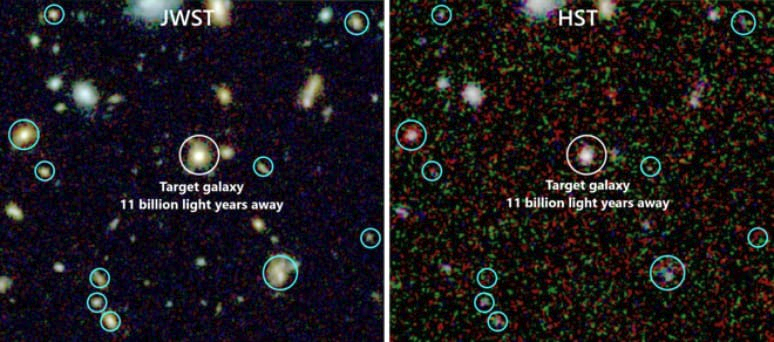
\includegraphics[scale=0.4]{targetGalaxy.png}
\end{figure}
\end{frame}


\begin{frame}{Seleção de Conjunto Alvo}
%Parâmetros:

%\begin{itemize}
%\tightlist
%\item
  %Cardinalidade miníma.
%\item
 % Maior tempo de ativação.
%\item
 % Maior peso.
%\item
 % Maior número de vértices ativados.
%\end{itemize}

Função limite, \(\forall v\in V\):

\begin{itemize}
\tightlist
\item
  Proporcional: \(0<p<1\) e \(f(v)=p\times d(v)\).
\item
  Majoritária ou Majorada: \(f(v)=\lceil\frac{d(v)}{2}\rceil\).
\item
  {\bf K-Limitada ou Linear}: Constante inteira \(k\) e \(f(v)=k\) ou
  \(f(v)=min(d(v),k)\).
\end{itemize}
\end{frame}

\begin{frame}{Seleção de Conjunto Alvo: NP-Díficil}


\begin{itemize}
\tightlist
\item NP-Díficil para grafos gerais {[}Chen 2009{]}
\item
  Tratável para alguns casos particulares {[}Dreyer et al.~2009, Centeno
  et al.~2011, Bollobás 2010, Chen 2009{]}
\item
  NP-Díficil com função limite Proporcional e Majoritária {[}Peleg et al.~1998, Chen 2009{]}
\item
  NP-Díficil com função $k$-Limitada ou Linear, mesmo se $k=2$ {[}Dreyer et al.~2009, Centeno et al.~2011,
  Bollobás 2010, Chen 2009{]}
\end{itemize}

%Explorar problemas NP-difícil:

%\begin{itemize}
%\tightlist
%\item
  %Complexidade parametrizada
%\item
 % Isolar e estudar casos polinomiais
%\item
 % Soluções exponenciais para pequenas entradas
%\item
 % Soluções aproximadas
%\item
 % Soluções heurísticas
%\end{itemize}
\end{frame}

\begin{frame}{Seleção de Conjunto Alvo: trabalhos relacionados}

\begin{columns}[T]
\begin{column}{.5\textwidth}

Kemp et al.~(2003):

\begin{itemize}
\tightlist
\item
  Maximização de influência em redes sociais
\item
  Heurísticas gulosas:

  \begin{itemize}
  \tightlist
  \item
    {\bf Maior contaminação}
  \item
    Maior grau
  \item
    Centralidade
  \item
    Aleatória.
  \end{itemize}
\end{itemize}
\end{column}
\begin{column}{.5\textwidth}
\centering
\begin{figure}
\centering
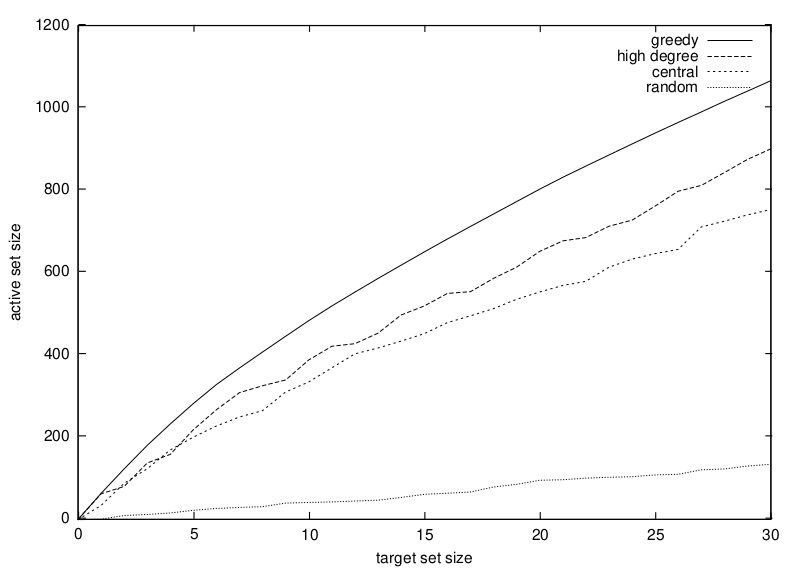
\includegraphics[scale=0.2]{img/kemp2003.png}
\end{figure}

\end{column}
\end{columns}

\end{frame}

\begin{frame}{Trabalhos relacionados}
\protect\hypertarget{trabalhos-relacionados}{}
\begin{figure}
\centering
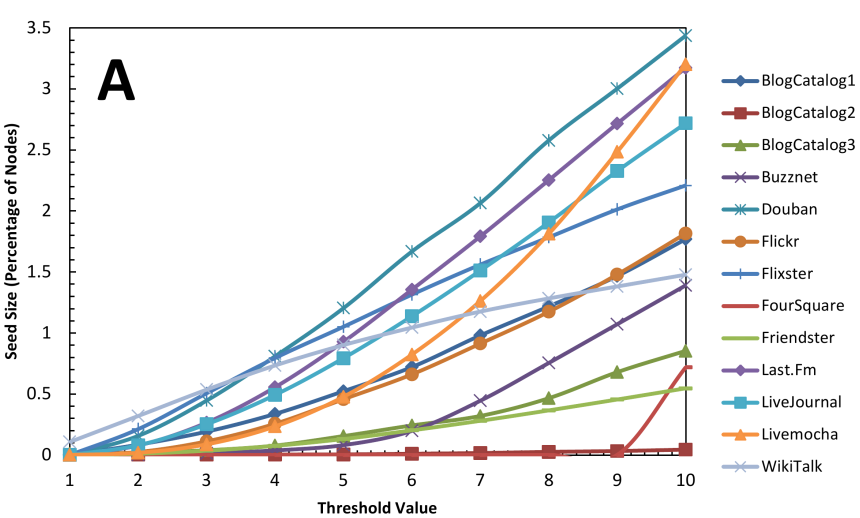
\includegraphics[scale=0.2]{img/shak1.png}
\end{figure}

Shakarian et al.~(2013):

\begin{itemize}
\tightlist
\item
  Experimento com mais de 30 redes sociais.
\item
  Programação Linear Inteira.
\item
  Explorou conjunto alvo com função k-limitado, função proporcional e tempo de ativação.
\end{itemize}
\end{frame}

\begin{frame}{Trabalhos relacionados - Shakarian et al.~(2013)}
\begin{columns}[T]
\begin{column}{.5\textwidth}
Algoritmo heurístico TIPDecomp:

\begin{itemize}
\tightlist
\item
  A cada iteração escolhe \(v\) não marcado com a menor
  relação \(d(v)-f(v)\).
\item
  Remove \(v\) do grafo.
\item
  Atualiza o grau dos vértices dos vizinhos de \(v\), marca os vértices
  \(u\) com \(d(u)<f(u)\).
\item
  Ao final os vértices não removidos são um conjunto alvo.
\end{itemize}

\end{column}
\begin{column}{.5\textwidth}
\centering
\begin{figure}
\centering
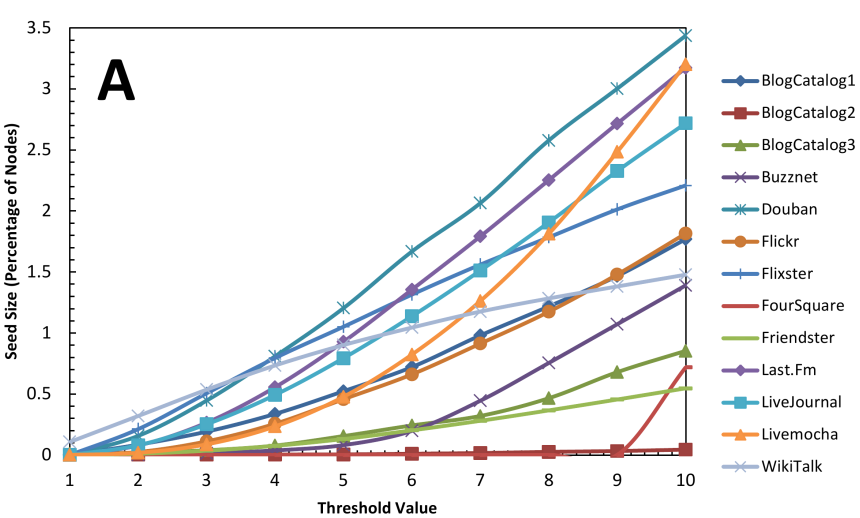
\includegraphics[scale=0.2]{img/shak1.png}
\end{figure}

\end{column}
\end{columns}
\end{frame}

\begin{frame}{Trabalhos relacionados}
\protect\hypertarget{trabalhos-relacionados-2}{}
Dinh (2014):

\begin{itemize}
\tightlist
\item
  Experimento com 3 redes sociais.
\item
  Realizou experimentos com heurísticas tradicionais tais como Kemp e
  apontou dificuldades:

  \begin{itemize}
  \tightlist
  \item
    Baixa qualidade dos primeiros vértices selecionados.
  \item
    Execução pouco escalável para redes sociais grandes.
  \end{itemize}
\item
  VIRAds: Algoritmo heurístico proposto.
\end{itemize}
\end{frame}

\begin{frame}{Trabalhos relacionados}
\protect\hypertarget{trabalhos-relacionados-3}{}
\begin{figure}
\centering
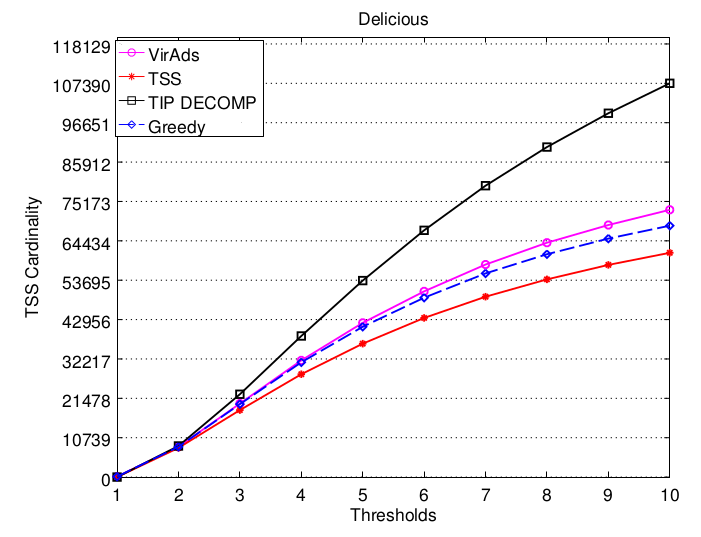
\includegraphics[scale=0.2]{img/cordasco.png}
\end{figure}

Cordasco et al (2018):

\begin{itemize}
\tightlist
\item
  Experimento com 13 redes sociais de Shakarian (2013)
\item
  TSS: Algoritmo de aproximação para o problema de seleção de conjunto
  alvo.
\item
  Explorou conjunto alvo k-limitado e comparou com Shakarian e Dinh.
\end{itemize}
\end{frame}

\begin{frame}{Trabalhos relacionados}
%\begin{figure}
%\centering
%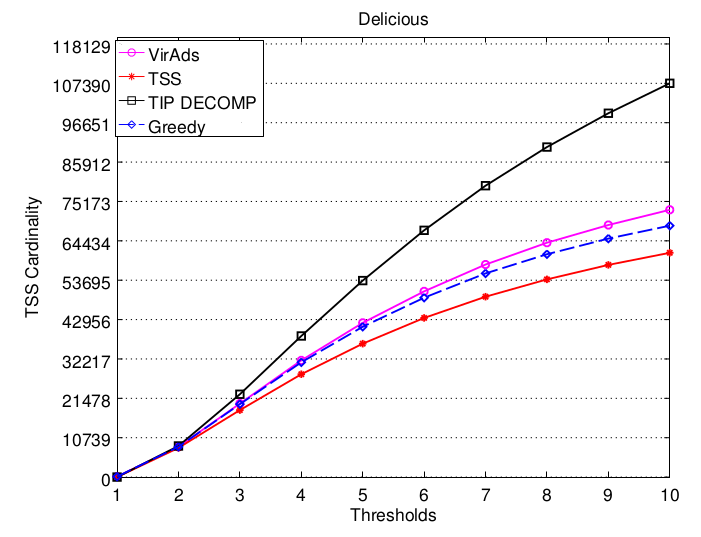
\includegraphics[scale=0.2]{img/cordasco.png}
%\caption{bg right:40\% fit}
%\end{figure}

Algoritmo TSS - Cordasco et al (2018):

\begin{itemize}
\tightlist
\item
  A cada iteração escolhe o vértice \(v\) com a maior relação
  \(\frac{f(v)}{d(v)(d(v)+1)}\).
\item
  Remove o vértice \(v\) do grafo e atualiza o grau e a função limite
  dos vértices dos seus vizinhos.
\item
  Adiciona os vértices \(u\) com \(d(u)<f(u)\) ao conjunto alvo.
\end{itemize}
\end{frame}

\begin{frame}{Seleção de Conjunto Alvo: Resumo heurísticas}

\textbf{Grau}: Nessa heurística a escolha de um novo vértice a ser incluído no conjunto alvo é sempre o vértice de maior grau.

\textbf{TIPDecomp}: Nessa abordagem, o grafo é decomposto, excluindo
vértices até que os vértices restantes sejam um conjunto alvo.

\textbf{TSSC}: Neste algoritmo o grafo é decomposto, eliminando vértices
até obter um grafo vazio. A medida que os vértices são retirados eles
são testados para compor o conjunto alvo. 

\textbf{Delta}: Escolhe o vértice disponível que trás o maior ganho marginal. Algumas variações
incluem como critério de desempate a contaminação parcial de mais vértices.
\end{frame}

\begin{frame}{Banco de grafos utilizados neste trabalho}
\begin{itemize}
\tightlist
\item
  Aleatórios de {[}Gilbert 1959{]}, de 5 até 100 vértices variando de 5
  com densidade variando de 0.1 até 0.9
\item
  Grafos de interesse.
\item
  Redes sociais:

  \begin{itemize}
  \item
    Intersecção Shakarian e Cordasco: 13 grafos
  
  \end{itemize}
\end{itemize}
\end{frame}

\begin{frame}{Parâmetros utilizados neste trabalho}
\protect\hypertarget{paruxe2metros}{}
\begin{itemize}
\tightlist
\item
  \(degree\): \(d(v)\) é o grau do vértice.
\item
  \(difficulty\): \(f(v)-d_C(v)\) é a dificuldade de contaminar o
  vértice.
\item
  \(dist\): \((d(v)-f(v))-d_C(v)\) é a diferença entre o grau do vértice
  e seu limite de ativação, descontado os vizinhos já ativados.
\item
  \(\Delta\): \(I^*[S\cup\{v\}] \setminus I^*[S]\) novos vértices
  ativados ao contaminar o vértice \(v\).
\item
  {\bf distDelta}: \(\sum_{i\in \Delta}((d(i) - t(i))-d_C(i))\) a soma da
  \(dist\) dos vértices de \(\Delta\).
\item
  {\bf difDelta}: \(\sum_{i\in \Delta}(t(i)-d_C(i))\) soma da dificuldade
  dos vértices de \(\Delta\).
\end{itemize}
\end{frame}

\begin{frame}{Nossa Heurística para Conjunto Alvo k-limitado}
\begin{itemize}
\tightlist
\item
  Divide o trabalho nas componentes conexas
\item
  Os vértices são iterados por ordem descendente de grau
\item
  O melhor vértice maximiza \(distDelta\) com desempate pelo maior
  \(difDelta\).
\item
  Todo vértice pertencente ao \(\Delta\) são podados da iteração atual.
\item
  Refinamento do resultado final transforma o conjunto alvo em minimal
\end{itemize}

%\begin{figure}
%\centering
%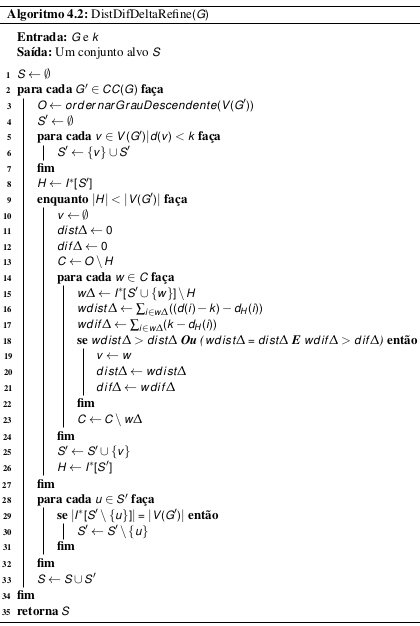
\includegraphics[scale=0.2]{img/algo-distdifdelta.png}
%\end{figure}
\end{frame}

\begin{frame}{Resultados: Conjunto alvo k-limitado}
\protect\hypertarget{resultados-conjunto-alvo-k-limitado}{}
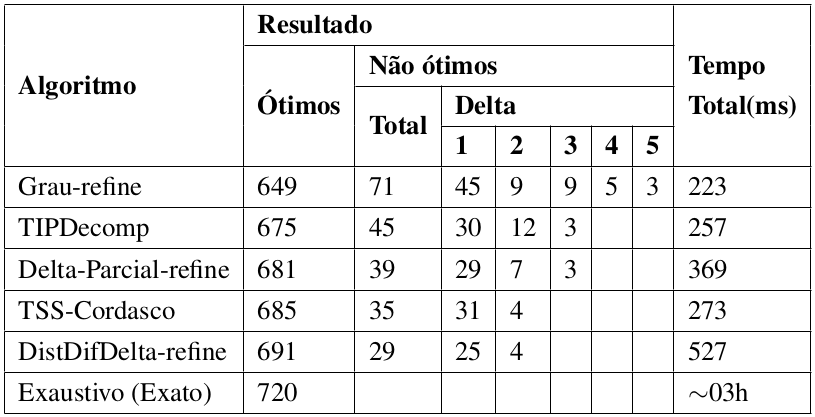
\includegraphics[scale=0.3]{img/alg-distdif-exato.png}
\end{frame}

\begin{frame}
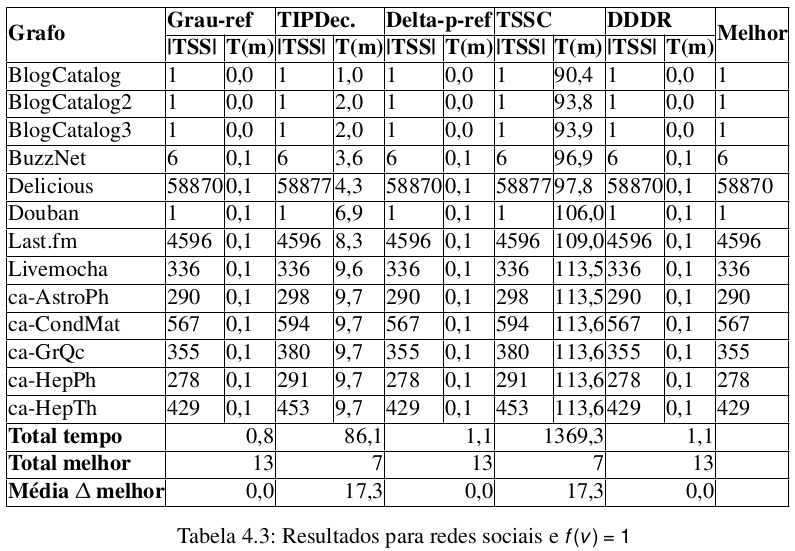
\includegraphics[scale=0.3]{img/k1.png} 
\end{frame}

\begin{frame}
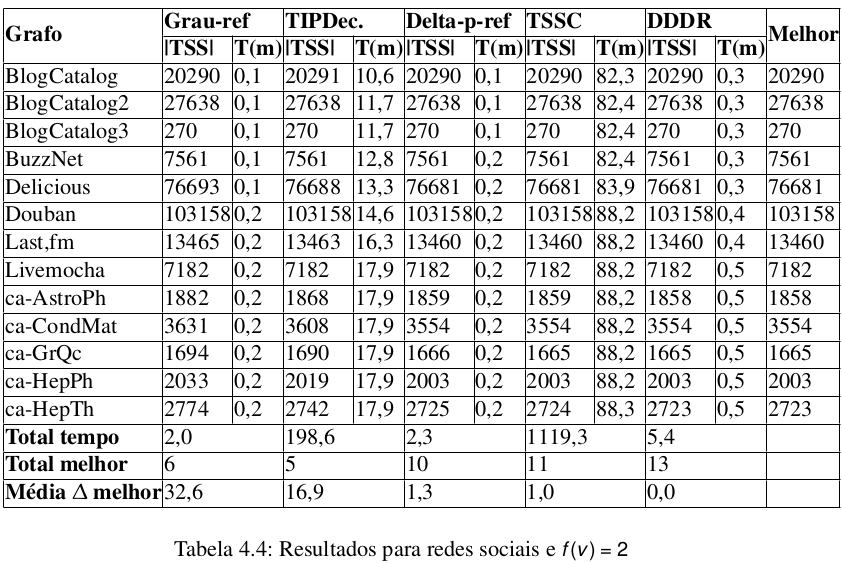
\includegraphics[scale=0.3]{img/k2.png}
\end{frame}

\begin{frame}
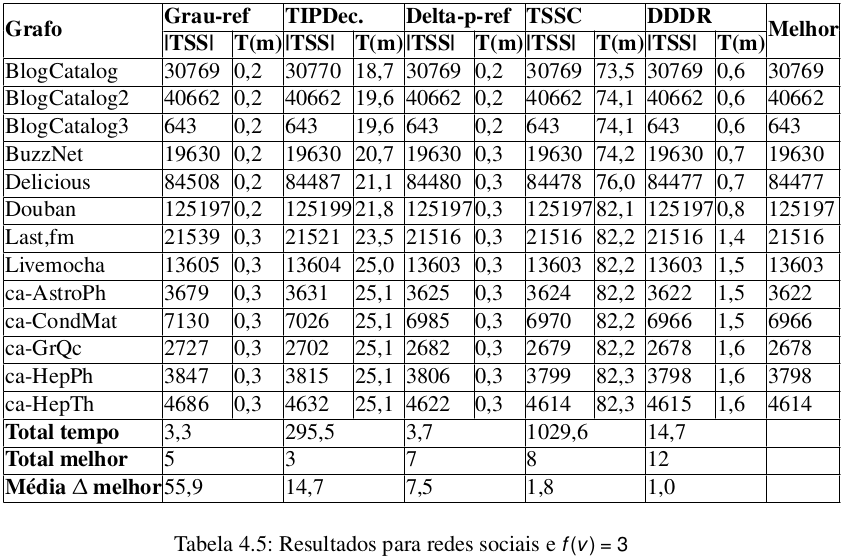
\includegraphics[scale=0.3]{img/k3.png} 
\end{frame}

\begin{frame}
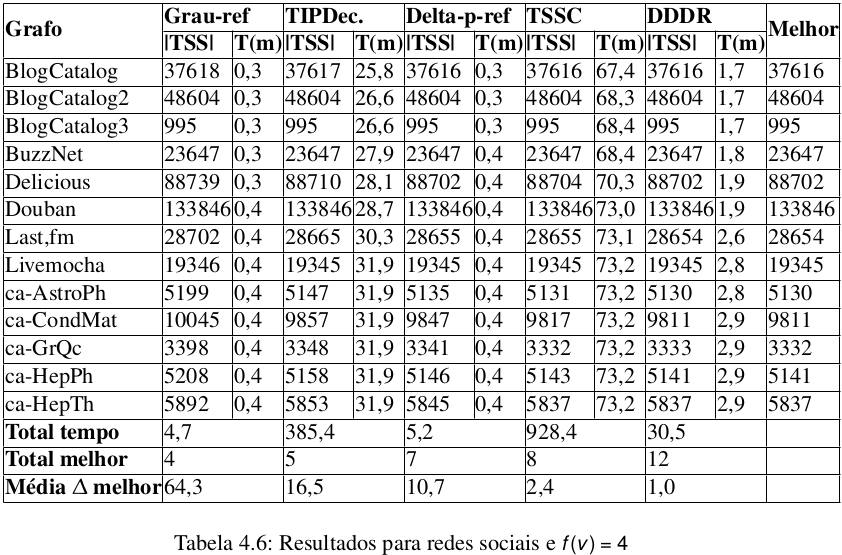
\includegraphics[scale=0.3]{img/k4.png}
\end{frame}

\begin{frame}
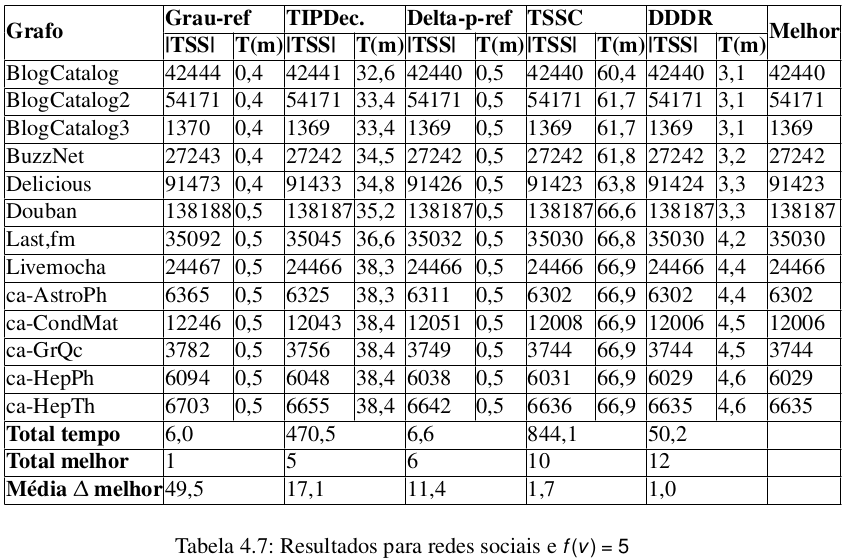
\includegraphics[scale=0.3]{img/k5.png} 
\end{frame}

\begin{frame}
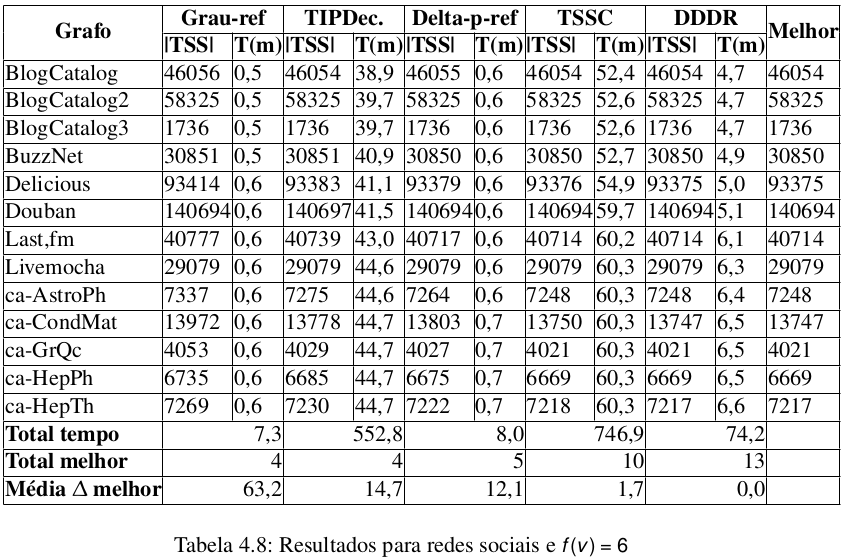
\includegraphics[scale=0.3]{img/k6.png}
\end{frame}

\begin{frame}{Resultados: Conjunto alvo k-limitado}
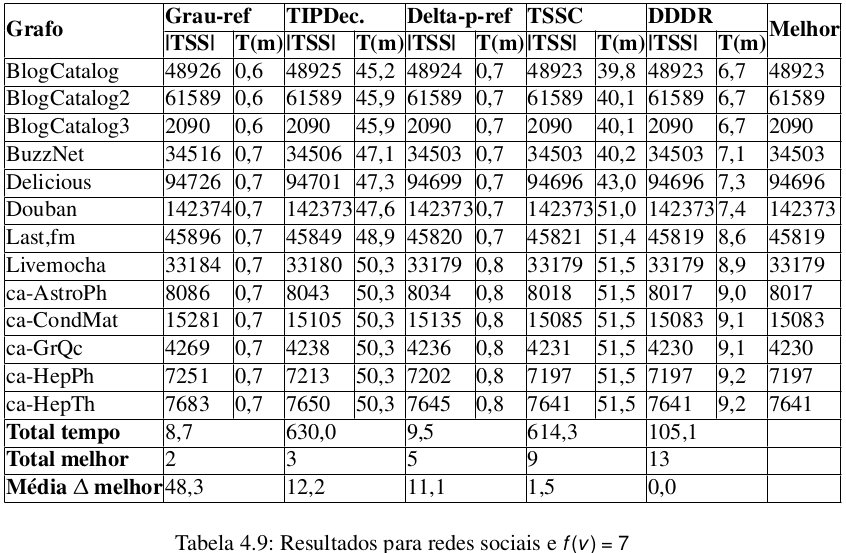
\includegraphics[scale=0.3]{img/k7.png}
\end{frame}

\begin{frame}{Algoritmo Exaustivo (exato)}
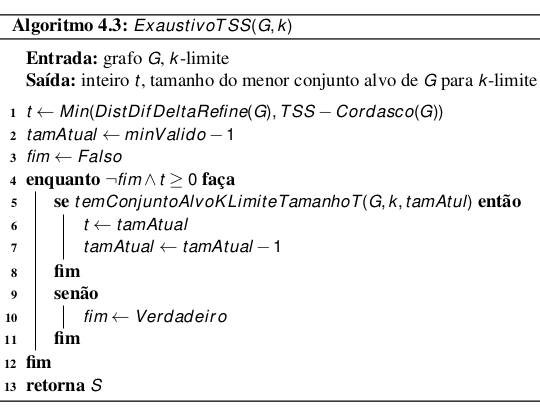
\includegraphics[scale=0.4]{img/algo-exaustivo.png}
\end{frame}

\begin{frame}{Resultados: Algoritmos exatos}
\begin{itemize}
\tightlist
\item
  Banco de dados de interesse
\item
  Modelo de programação linear
\end{itemize}

\begin{figure}
\centering
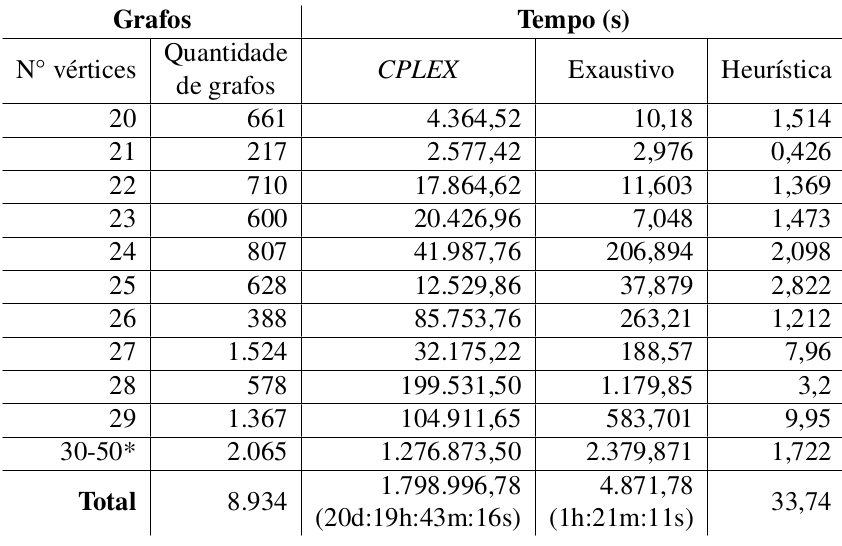
\includegraphics[scale=0.3]{img/comparativo-exato.png}
\end{figure}
\end{frame}

\begin{frame}{Considerações finais e trabalhos futuros}
Esperamos já ter relevantes contribuições para Heurística de Seleção de Conjunto alvo Majoritário.

\begin{itemize}
\tightlist
\item
  Demonstrar a exatidão dos algoritmos para algumas classes de grafos.
\item
  Trabalho consolidado para um periódico:

  \begin{itemize}
  \tightlist
  \item
    Contemplar resultados k-limitado
  \item
    Estender o banco de grafos avaliados
  \item 
  Expandir os resultados para bancos de grafos maiores e mais diversificados. 
 \end{itemize}
\end{itemize}
\end{frame}

\begin{frame}{Referências}
\protect\hypertarget{referuxeancias}{}
\begin{itemize}
\item
  Centeno et al.~2011: Irreversible conversion of graphs. Theoretical
  Computer Science, Elsevier B.V., v. 412, n.~29, p.~3693--3700, 2011.
\item
  Chen et al.~2009: Efficient influence maximization in social networks.
  Proceedings of the 15th ACM SIGKDD International Confe- rence on
  Knowledge Discovery and Data Mining.
\item
  Cordasco et al.~2018: Discovering Small Target Sets in Social
  Networks: A Fast and Effective Algorithm. Algorithmica, v. 80, n.~6,
  p.~1804--1833, 2018.
\item
  Dinh et al.~2014: Cost-effective viral marketing for time-critical
  campaigns in large-scale social networks. IEEE/ACM Transactions on
  Networking, v. 22, n.~6, p.~2001--2011, 2014. ISSN 10636692.
\end{itemize}
\end{frame}

\begin{frame}{Referências}
\protect\hypertarget{referuxeancias-1}{}
\begin{itemize}
\item
  Dreyer e Roberts 2009: Irreversible k-threshold processes:
  Graph-theoretical threshold models of the spread of disease and of
  opinion. Discrete Applied Mathematics, Elsevier B.V., v. 157, n.~7,
  p.~1615--1627, 2009. ISSN 0166218X.
\item
  Kemp et al.~2003: Maximizing the spread of influence through a social
  network. Proceedings of the Ninth ACM SIGKDD International Conference
  on Knowledge Discovery and Data Mining.
\item
  Peleg 1998: Size bounds for dynamic monopolies. Discrete Applied
  Mathematics, v. 86, n.~2, p.~263--273, 1998. ISSN 0166-218X.
\end{itemize}

Imagens:

\begin{itemize}
\tightlist
\item
  Wikimedia Grafos
\item
  WikWiley Knowledge-Discovery-1942-4795
\item
  Itcilo: Social Network Analysis
\end{itemize}
\end{frame}

\begin{frame}{Fim}
\protect\hypertarget{fim}{}
\begin{itemize}
\tightlist
\item
  Obrigado!
\item
  Dúvidas?
\end{itemize}
\end{frame}

\end{document}
